% Kapitola Teorie
\chapter{Teoretická východiska práce}

\begin{chapterabstract}
	V této kapitole se budeme zabývat teoretickými východisky práce a vymezením používaných pojmů.
	 Také si ukážeme existující řešení problémů podobných našemu.
	 TODO Doplnit abstract Teorie
\end{chapterabstract}

\section{Analýza sentimentu}
Na poli výzkumu dolování dat z textu můžeme narazit na dva pojmy, které jsou zaměnitelné. Jedná se o \textit{Analýzu sentimentu (SA)} a \textit{Opinion mining (OM)}. \cite{Medhat} Někteří autoři je ale rozlišují. Například Tsytsarau a Palpanas uvádějí \cite{survey}, že OM extahuje a analyzuje názor lidí vázající se k nějakému objektu či entitě, kdežto SA pouze identifikuje sentiment vyjádřený v textu a ten pak analyzuje. \marginpar{\todo{pozn. redakce: Víc mi teda sedí to vyjádření že SA a OM jsou jiné, ale uvidim}}
Podle Medhata a spol. můžeme SA rozdělit na 3 klasifikační úrovně \cite{Medhat}:
\begin{description}
	\item[Document-level] Základní jednotkou informace je jeden dokument (týkající se jednoho tématu)

	\item[Sentence-level] Určuje sentiment na základě jedné věty. 
	
	\item[Aspect-based] Určuje sentiment s ohledem na entity a jejich aspekty, kde autoři názoru mohou poskytovat různé názory na různé aspekty jedné entity (např. \uv{V této firmě se necítím dobře, ale platové podmínky jsou nejlepší na trhu}).
\end{description}

Feldman k těmto úrovním přidává ještě další 2 \cite{Feldman}:
\begin{description}
	\item[Komparativní] Základní jednotkou informace je jeden dokument (týkající se jednoho tématu)
	
	\item[Lexicon acquisition] Určuje sentiment na základě jedné věty. Není nijak zvláště rozdílná od Dokument-level analýzy, protože věty jsou v principu jen krátké dokumenty. 
	
\end{description}

\subsection{Document-level}
Jedná se o nejjedodušší formu SA. Jak již bylo řečeno, základní jednotkou informace této metody je jeden dokument a předpokládá se, že zde autor vyjadřuje svůj názor na jeden objekt. Existují dva hlavní přístupy řešení a to: supervizované a nesupervizované učení. Supervizované učení v tomto případě předpokládá, že existuje konečná množina tříd, reprezentující hledaný sentiment.  V nejjedodušším případě si vystačíme s 2 třídama, konkrétně negativní a pozitivní sentiment. Obecně se tak jedná o nějakou diskrétní škálu hodnot. 
Nesupervizované učení využívá Semantic orientation (dále jen SO) \todo{SO = kapitola?} konkrétních slov nebo vět. 
\subsection{Sentence-level}
Pokud problém vyžaduje detailnější analýzu, než poskytuje Document-level, využijeme Sentence-level metodu. Prvotně musíme věty rozdělit na subjektivní a objektivní. Objektivní věty se pro další analýzu často nevyužívají, ale některé přístupy využívají oba typy vět. Po rozdělení můžeme opět využít buďto supervizované nebo nesupervizované učení, stejně tak jako u Dokument-level analýzy.
Narayanan a spol. ukázali, že je vhodné na různé věty používat různé metody \cite{Feldman24}. Konrétně věty různých typů: tázací, podmiňovací a sarkastické. 
\subsection{Aspect-level}
Předchozí 2 typy byly předpokládaly že se každý dokument nebo věta váže k jednomu objektu. V mnoha případech však lidé hovoří o více objektech s více aspekty (objektem může být např. mobilní telefon, u kterého se můžeme vyjádřit k jeho aspektům (rychlost, velikost, paměť, atd.) kladně i záporně). Kdybychom analyzovali text o jednom objektu s více aspekty těmito přístupy, došlo by ke ztrátě mnoha informací. Aspect-level analýza se proto zaměřuje v na jednoltlivé aspekty objektu a k nim přiřazuje zjištěný sentiment. 

Nejdříve tedy musíme identifikovat aspekty objektu. Většina komerčních produktů používá přístup, kde si nejdříve vyfiltrují všechny fráze s podstatnými jmény (dále je n NPs -noun
phrases), kterých je určitý počet. \cite{Feldman} Dále pak můžeme zredukovat šum v NPs \todo{cite Feldman30} pomocí PMI \todo{PMI}. Existují ale i další přístupy: Například phrase dependency parser, Conditional Random Field, atd. Tyto metody identifikují takzvané explicitní aspekty, ale v textu se mohou nacházet i implicitní aspekty (např. ve větě: \uv{Toto auto je pomalé} není nikde uveden aspekt rychlosti).\todo{implicit metody} \uv{Finální polarita každého aspektu je determninována váženým průměrem polarit všech výrazů sentimentu nepřímo vážené vzdálenopsti  mezi aspektem a výrazem sentimentu.} \cite*[překlad vlastní]{Feldman}

\subsection{Komparativní analýza}
V některých případech se lidé nevyjadřují k objektech příme, ale porovnávají 2 objekty mezi sebou (např. \uv{Windows je lepší operační systém, než jakákoliv distribuce Linuxu}). Zde tedy musíme vyextahovat objekty z těchto vět. Autorům Jindal a Jiu se podařilo najít relativně malou množinu slov, která tyto věty dokáže identifikovat. \cite{comparative} Jedná se o anglické slova, například o: \cite{comparative} 
\begin{description}
	\item[Srovnávací přídavná jména a příslovce] \uv{more} - více, \uv{less} - méně a slova končící koncovkou \uv{-er}

	\item[Přídavná jména a příslovce v superlativu]  \uv{most} - nejvíce, \uv{least} - nejméně a slova končící koncovkou \uv{-est}
	
	\item[Jiné fráze] \uv{than} - než, \uv{outperform} - překonat, \uv{up against} - proti, $\dots$
\end{description}
\uv{Tyto klíčová slova a fráze (celkem 83) dokáží zachytit komparativní věty se senzitivitou $94\%$}. \cite[překlad vlastní]{comparative}


\subsection{Lexicon acquisition}
\blind[2]
		
\section{Metodika analýzy}

Analýza sentimentu si můžeme představit jako proces. Na obrázku \ref{fig:SAprocess} můžeme vidět její součásti. Data nejčastěji bývají z recenzí produktů, avšak to mohou být i novinové články nebo politické debaty. \cite[překlad vlastní]{Medhat}. Ve fázi identifikace sentimentu vybíráme možné slova nebo fráze vyjadřující názor. Následuje výběr příznaků a klasifikace sentimentu, kde existuje více přístupů. \cite[překlad vlastní]{Medhat} 


\begin{figure}[h]
    \centering
    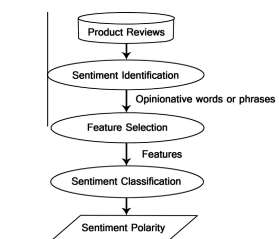
\includegraphics[height=5cm]{text/img/SAProcess.PNG}
    \caption{\todo{Přeložit do češtiny a popisek.}}
    \label{fig:SAprocess}
\end{figure}

Tyto přístupy můžeme rozdělit na dvě základní skupiny: strojové učení a přístup založený na slovníku.

\subsection{Přístupy strojového učení}

Strojové učení se běžně rozděluje na tyto skupiny: \cite{ml1} 

\begin{description}
	\item[Supervizované učení] - Máme k dispozici vstupní data (příznaky) a k nim přiřazený správný výstup (ten může být diskrétní resp. spojitý a potom úlohu nazýváme klasifikační resp. regresní). Díky označeným datům, můžeme trénovat náš model, na základě chyb od originálního výstupu. Data se zde rozdělují do 3 skupin: trénovací, validační, testovací v určitém poměru (zde se zdroje neschodují na stejných hodnotách, většinou se ale jedná o poměr 3:1:1 viz. Obrázek \ref{fig:datasplit}). Trénovací slouží k trénování modelu a jeho parametrů, validační k jeho porovnání s ostatními natrénovanými modely a testovací pak k odhadu chyby našeho modelu. 
	\item[Nesupervizované učení] - Zde nemáme ke vstupním datům odpovídající výstup a autor zde musím sám najít souvislosti. 
	\item[Semi-supervizované učení] - Kombinace supervizovaného a nesupervizovaného učení
	\item[Posilované učení] -  Ayodele jej definuje takto: \uv{Algoritmus se učí pravidla, jak jednat při pozorování světa. Každá akce má nějaký dopad na prostředí a prostředí poskytuje zpětnou vazbu, která řídí algoritmus učení.} \cite[překlad vlastní]{ml1} 
	
	\item[A další] 
\end{description}


\begin{figure}[h]
    \centering
    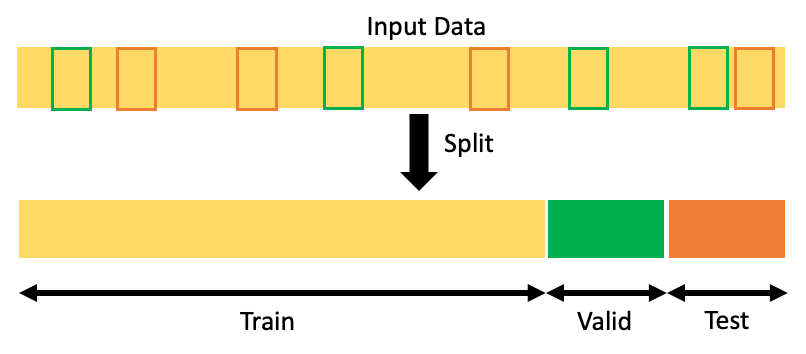
\includegraphics[height=5cm]{text/img/data.png}
    \caption{\todo{Přeložit do češtiny a popisek.}}
    \label{fig:datasplit}
\end{figure}

Medhat ve svém článku ukázal používáné metody z jiných článků zabývajících se analýzou sentimentu. \cite{Medhat} Výčet z kategorie strojového učení pak můžeme vidět na Obrázku \ref{fig:MedhatML}. V následujících kapitolách si tyto metody/modely představíme.

\begin{figure}[h]
    \centering
    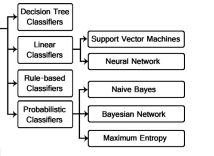
\includegraphics[height=3cm]{text/img/medhatML.PNG}
    \caption{\todo{Přeložit do češtiny a popisek.}}
    \label{fig:MedhatML}
\end{figure}

\subsubsection*{Rozhodovací stromy}
Rozhodovací strom je jednoduchý model, který můžeme použít ke klasifikaci i regresi. Kotsiantis jej definuje takto: \uv{Rozhodovací stromy jsou sekvenční modely, které postupně provádějí jednoduché testy, porovnání;
každý test porovnává číselný atribut s prahovou hodnotou nebo s nominálním atributem
soubor možných hodnot.} \cite[překlad vlastní]{decisionTree} Russel a Norvig jej zase definují obecněji jako \uv{funkci, která jako vstup očekává vektor příznaků a vrací jednu hodnotu -- rozhodnutí}. \cite[překlad vlastní]{aimodern} Oproti jiným modelům jsou rozhodovací stromy také lépe graficky reprezentované (pomocí stromové struktury viz obrázek 
\ref{fig:decisionTree}) a rychlé k pochopení. Výsledek klasifikaci resp. regrese k určitým příznakům zjistíme z daného listu, do kterého se vstupní data postupním porovnáváním listu \textit{dostala}. 



\begin{figure}[h]
    \centering
    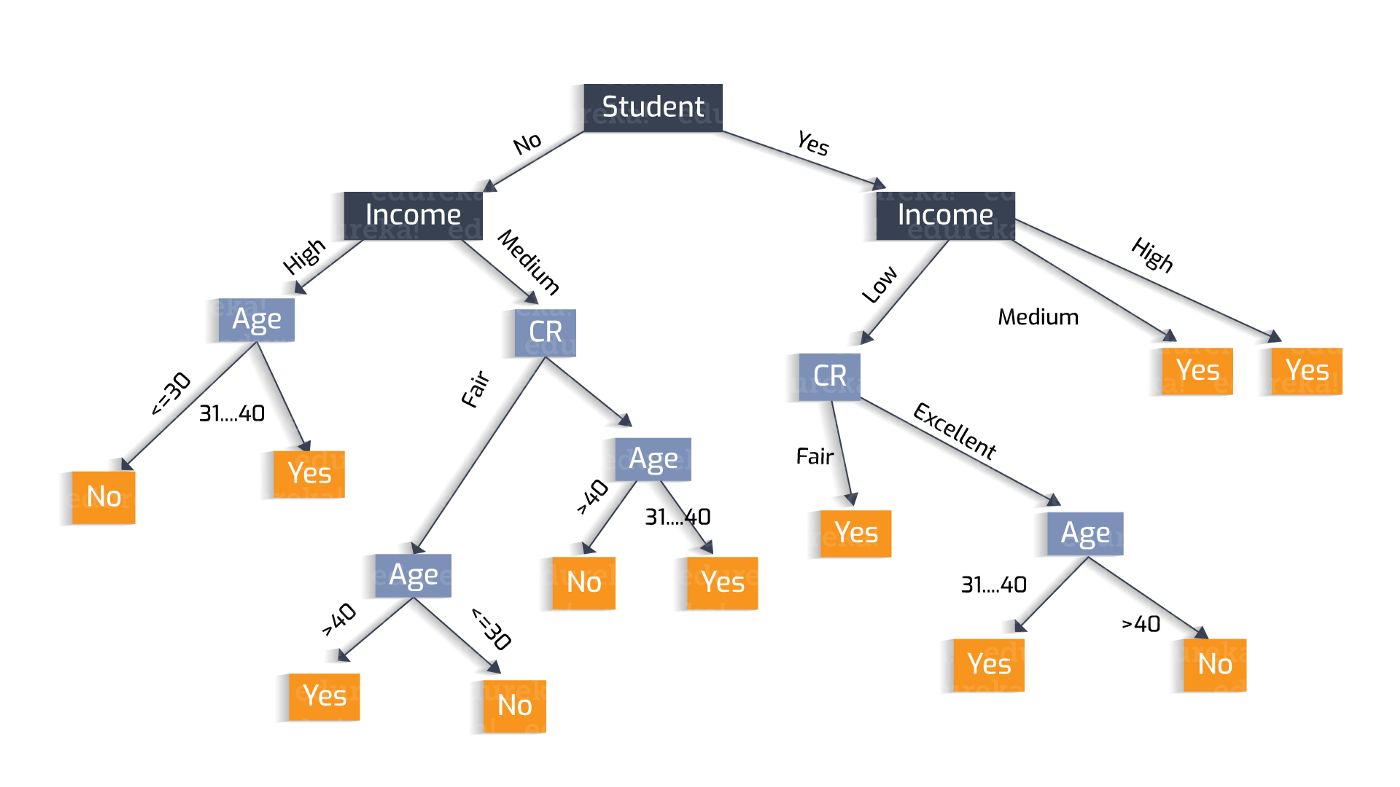
\includegraphics[height=5cm]{text/img/decisionTree.png}
    \caption{\todo{Přeložit do češtiny a popisek.}}
    \label{fig:decisionTree}
\end{figure}

Než vysvětlíme jak stromy vytvářet, budeme k tomu potřebovat různé metriky, pomocí kterých určíme kvalitu rozdělení vektoru příznaků podle určité podmínky.

\todo{Trochu přeformulovat}
Jednou z metrik je tzv. \textbf{informační zisk} a vypočítáme ho jako\cite{decisionTrees}:
\[
InformacniZisk(\mathcal{D},X_i) = IG(\mathcal{D}) = H(\mathcal{D}) - \sum^{k-1}_{j = 0} t_j  H(\mathcal{D}_j),
\]kde $\mathcal{D}_j$ je podmnožina $\mathcal{D}$ pro které $X_i = j$, $t_j$ je podíl počtu prvků v $\mathcal{D}_j$ a $\mathcal{D}$. 

Funkce $H(\mathcal{D})$ ve vzorci je pak odhad entropie dat:
\[
Entropie(\mathcal{D}) = H(\mathcal{D}) = - \sum^{k-1}_{i = 0} p_i  \log(p_i),
\]
kde $\mathcal{D}$ je množina dat, $p_i$ je  poměr počtu $i$ v $\mathcal{D}$ a platí $ \sum^{k-1}_{i = 0} p_i = 1$. 


Další metrikou je tzv. \textbf{Gini index}, která udává míru toho, že nově přidaný prvek bude špatně klasifikován. Přesný výpočet je \cite{vzd}:
\[
GiniIndex(\mathcal{D}) = GI(\mathcal{D}) = \sum^{k-1}_{i = 0} p_i  (1 - p_i) 
\]
Gini index můžeme využit při výpočtu informačního zisku, kdy jen ve vzorci nahradíme $(\mathcal{D})$ za  $GI(\mathcal{D})$.


Narozdíl od paramestrů, které hledáme při trénování (parametry = vrcholy, trénování = konstrukce stromu),  má rozohodovací strom hyperparametry. Hyperparametry modelu jsou takové parametry, které se používají při konstrukci stromu. Určují používané metriky a hodnoty podmínek větvení, resp. vytváření listů. Hledání nejoptimálnějších hodnot se nazývá \textbf{ladění hyperparametrů} a jedná se o systematické zkoušení různých kombinací hodnot a vyhodnocování výsledků modelu. Mezi základní hyperparametry patří \cite{scikit-learn}:
\begin{description}
\item[Kritérium] -- Funkce, která měří kvalitu rozdělení příznaků. Nejčastější jsou Gini index nebo Entropie. Tato funkce se pak použije při výpočtu informačního zisku.
\item[Maximální hloubka] -- Maximální hloubka rozhodovacího stromu. V každém úplném binárním stromě s hloubkou $h$ je přesně $2^{h-1}$. Kdybychom měli $h$ příznaků \footnote{Opět pro jednoduchost uvažujeme binární klasifikaci.}, tak počet všech možnách kombinací je také $2^{h-1}$, čímž by strom \uv{degradoval} na slovník. Díky tomuto hyperparametru můžeme této \uv{degradaci} předejít.
\item[Váha příznaků] -- Slouží k vážení důležitosti příznaku.
\item[Minimální počet výsledků v listu] --  Pokud při konstrukci stromu není dostatek příznaků, vytvoří se list.
\end{description} 

K vytváření stromů pak existují algoritmy. Známý je ID3, který konstruuje stromy pomocí hladového přístupu. Jeho nevýhodou je předpoklad diskrétních dat a absence chybějích hodnot. Také se na malých datasetech přeučuje. 

\begin{algorithm}[h]

    \SetKwInput{Vst}{Vstup}
    \SetKwInput{Vyst}{Výstup}
    
    \Vst{Matice příznaků, vektor vysvětlované proměnné}
    
    \Vyst{Rozhodovací strom}
    
    
     \uIf{žádná data}
     {
        \Return fail list
     }
     \uElseIf{$\forall$ příklady mají stejný výsledek}
     {
        \Return list, který vrací výsledek klasifikace
     }
     \uElseIf{je splněna podmínka hyperparametru}
     {
        \Return list, který vrací výsledek klasifikace
     }
     \Else
     {
        A $\leftarrow$ příznak nejlépe rozdělující vektor výsledků\;
        r, l  = split(A,X,y)\;
        levý\_syn $\leftarrow$ ID3(rX,rY)\;
        pravý\_syn $\leftarrow$ ID3(lX,lY)\;
     }
    
     \caption{Iterative Dichotomiser 3}
     \label{id3}
    \end{algorithm}

Jeho vylepšení nástupci C4.5 a C5.0, kteří už dokážou pracovat i se spojitými daty i chybějícími hodnotami. Od svého předchůdce se liší technikou \textbf{prořezávání}, při které po konstrukci stromu prochází a odstraňuje zbytečné větve. Tato technika nám pomůže proti přeučení stromu. Existují dva druhy prořezávání, a to pre-prořezávání (při zjištění nespolehlivé informace přestaneme dále rozvíjet současnou větev) a post-prořezávání (nejdříve se zkonstruuje strom a zbytečné části se odstraní).

Posledním algoritmem je CART nebo-li Classification And Regression Trees a je velice podobný algoritmu C4.5. Narozdíl od něj ale umí pracovat se spojitou vysvětlovanou proměnou (tj. regrese). \uv{\textit{CART konstruuje binární stromy pomocí prahových hodnot, které přinášejí největší zisk informací v každém uzlu.}}


\subsubsection{Naivní Bayesův klasifikátor}
Tento klasifikátor spadá do kategorie pravděbodobnostních klasifikátorů. Klasické klasifikátory jsou reprezentované funkcí, která mapuje vstup (vektor příznaků) na výslednou klasifikační třídu. Narozdíl od nich, pravděbodobnostní klasifikátory vrací podmíněnou pravděbodobnost $p(y|x)$, kde $y$ je výsledná třída  a $x$ je vektor příznaků.

\begin{definition}[Podmíněná pravděbodobnost]
    $$ p(y|x) = \frac{p(y,x)}{p(x)} $$
    \end{definition}

Existují dva přístupy, jak tuto pravděbodobnost dostat. \cite{naiveBayes} \uv{Prvním je přímo vytvořit funkci, která vypočítá určité pravděbodobnosti $p(y|x)$} \cite[překlad vlasntí]{naiveBayes}. Tento model pak nazýváme \textbf{diskriminativní}.

Druhým přístup nazýváme \textbf{generativní}. Pro každou hodnotu $y$ model naučíme $p(x|y)$ a $p(y)$. Poté budeme potřebovat Bayesovu větu \cite{prob}:

    \begin{definition}[Bayesova věta]
        Buďiž $a_1, a_2, \hdots, a_n$ vzájemně disjunktní náhodné jevy, jejichž sjednocení tvoří celý pravděbodobnostní prostor a platí: $\forall i : p(A_i) > 0 $. Pak pro libovný jev $b$ takový, že $p(b) > 0$, platí: 
        $$p(a_i|b) = \frac{p(a_i)p(b|a_i)}{p(b)} = \frac{p(a_i)p(b|a_i)}{\sum_{i=1}^{n}p(b_i|a)p(b_i)}$$
        \end{definition}

Po aplikování Bayesovy věty dostaneme chtěnou pravděbodobnost $p(y|x)$ \cite{naiveBayes}:

$$p(y|x) = \frac{p(x,y)}{p(x)} = \frac{p(x|y)p(y)}{\sum_{y' = 1}^{C}p(x|y')p(y')}$$
Označujeme ho generativním, protože představuje úplnou informaci o rozdělení, ze kterého byla data generována. Výslednou predikci klasifikační třídy pak určíme jako 
$$ Y = arg\,max_y p(y|x)$$

Klasifikátor nazýváme naivním, protože očekává nezávislost všech příznaků:
$$ p(x|y = c) = \prod_{i=1}^{D}p(x_i|y = c)$$
\uv{I přes to, že toto obvykle neplatí (příznaky jsou většinou závislé), výsledný model je jednoduché natrénovat a funguje překvapivě dobře.}\cite[překlad vlastní]{naiveBayes}
\todo{ODHADY PARAMETRŮ}

\subsubsection{Bayesovské sítě}

Bayesovské sítě jsou typem pravděpodobnostního grafického modelu, který pro výpočty pravděpodobnosti používá bayesovské odvození. Bayesovské sítě mají za cíl modelovat podmíněnou závislost, a tedy i kauzalitu, reprezentováním podmíněné závislosti hranami v orientovaném grafu.

Pro začátek si zadefinujeme pár pojmů. 

\begin{definition}[DAG - Orientovaný acyklický graf]
    Orientovaný graf G nazveme \textbf{acyklický}, pokud neobsahuje jako podgraf orientovanou kružnici.
    \end{definition}

    \begin{lemma}[Multiplikativní zákon]
        Pro jevy $a_1, a_2, \hdots, a_n$ platí: 
        $$p(a_1 \cap \hdots \cap a_n) = p(a_1)p(a_2|a_1)p(a_3|a_1 \cap a_2)\hdots p(a_n| a_1 \cap \hdots \cap A_{n-1}) $$
        \end{lemma}

        \begin{definition}[Podmíněná nezávislost]
            Buď jev $c$ náhodný jev s $p(c) > 0 $. Náhodné jevy $a, b$ jsou \textit{podmíněně nezávislé za podmínky c} pokud platí: 
            $$p(a \cap b|c) = p(a|c)p(b|c)$$
            \end{definition}
Bayesovská síť je  orientovaný acyklický graf, kde každý vrchol představuje náhodný jev a hrany mezi vrcholy představují podmíněné pravděbodobnosti. 

\subsubsection{Neuronové sítě}
Neuronové sítě se svojí strukturou inspirovali strukturou vzájemně propojených neuronů v biologických systémech. 

Základní stavební jednotkou je neuron, který:
\begin{itemize}
    \item Přijímá reálné vstupy
    \item Produkuje jeden výstup
\end{itemize}

Nejjednodušším modelem neuronové sítě určeným ke klasifikaci aje tzv. jednovrstvý perceptron (schéma viz. \ref*{fig:perceptron}).

\begin{figure}[h]
    \centering
    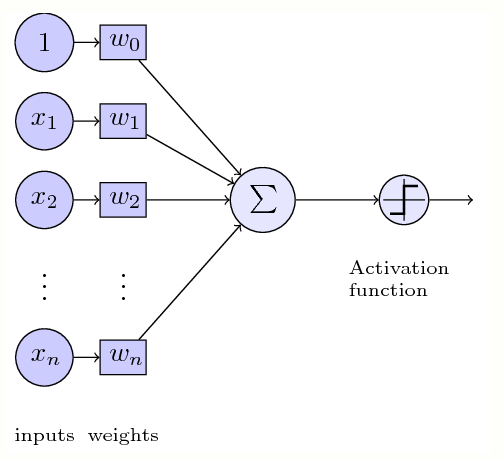
\includegraphics[height=5cm]{text/img/pereptron.PNG}
    \caption{\todo{Přeložit do češtiny a popisek.}}
    \label{fig:perceptron}
\end{figure}

Výstup neuronu se získá aplikací nelineární aktivační funkce f na hodnotu vnitřního potenciálu $\xi$ daného
součtem vstupů $x_1, \hdots , x_n$ pronásobených příslušnými vahami $w_1, \hdots , w_n$ a interceptu $w_0$. V případě perceptronu uvažujeme jako aktivační funkci tzv. skokovou funkci dánou předpisem:
$$f(\xi) = \begin{cases}1 & \text{když }\ \xi \geq 0,\\0 &\text{když} \xi < 0\end{cases} $$
\subsubsection{SVM}
\subsubsection{Maximální entropie}
\subsubsection{Ruled based?}